\section{Implementation}

The goals it to turn the raw data from the \cams into an image format that can be passed to the \gls{h265} encoder, namely the \code{P010_10LE} format.
\code{P010_10LE} is a YCbCr 4:2:0 format with with semi-interlaced data and 10 bits per channel stored in the most significant bits of 16 bit little-endian unsigned integers.

This transformation can be broken down into separating different angles of polarization, debayering the byer data, translate the resulting RGB data to YcbCr, perform chroma subsampling and package the data in the correct way.
This whole process is visualzed in Figure \ref{fig:transform}.

\begin{figure}[H]
    \centering
    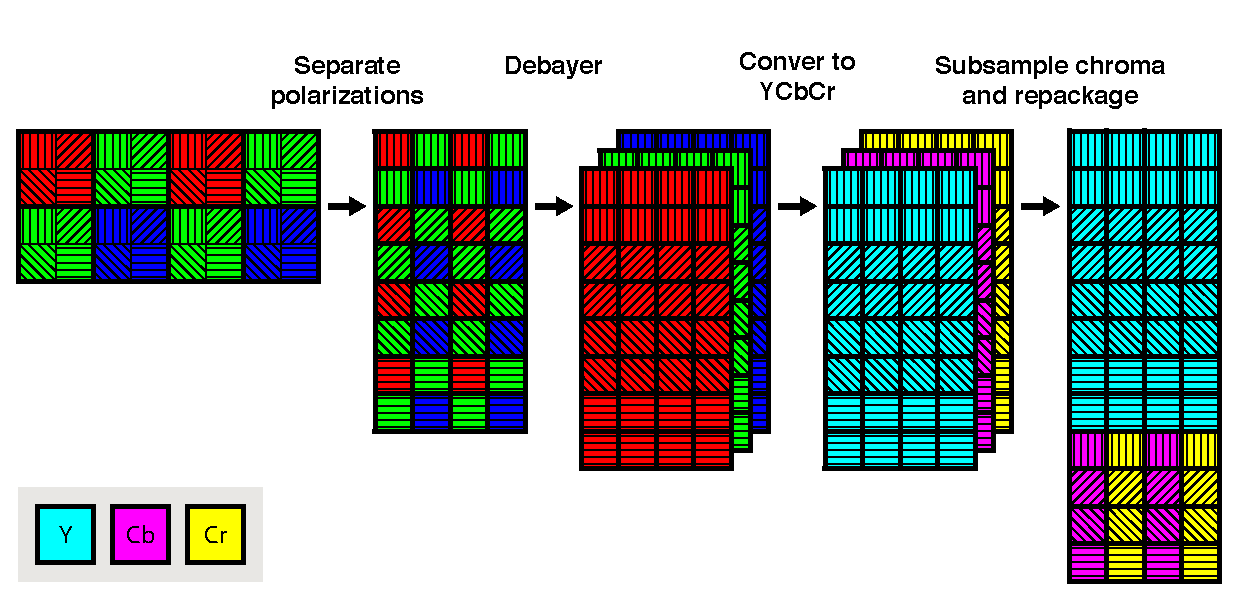
\includegraphics[width=\textwidth]{figures/polarized_image/transform.pdf}
    \caption{Visualization of how the raw custom bayer pattern is transforemd into a YCbCr format where the angles of polarization are stacked vertically.}
    \label{fig:transform}
\end{figure}

I initially tried solving the problem using \gls{numpy} and \gls{opencv}, as I knew that a CUDA implementation would not be trivial.
But, even when levraging all eight \gls{cpu} cores to their full extent it was not possible to perform all the steps fast enough to keep up with the video input from both cameras.
Running the \gls{cpu} cores at max frequency also had a big inpact on the power consumption of the \jx.



In order to acheive the highest possible throughput, this whole transformation process is more or less performed in a single step and several performance optimizations are performed.










